% !TEX root = ./Vorlesungsmitschrift DIFF 2.tex  
\chapter{Untermannigfaltigkeiten des \texorpdfstring{\( \reals^n \)}{R\^n}}
\lecture{Do  28.05. 10:15}{}
Ziel (\ua) Geometrische Interpretation der Ableitung.
\begin{erinnerung*}
  Der Gradient zeigt in die Richtung des stärksten Anstiegs.
  \begin{figure}[H]
    \centering
    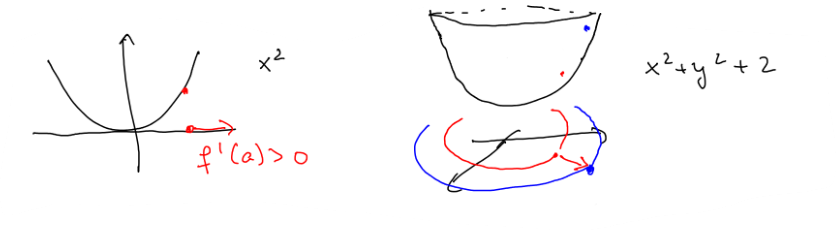
\includegraphics[width=0.8\linewidth]{erinnerung_gradient_intuition}
    \caption*{}
    \label{fig:erinnerung_gradient_intuition}
  \end{figure}
  In einem Beispiel hatten wir gesehen: Richtungsableitung in Richtung einer Niveaufläche steht \( \perp \) auf \( \grad-{f} \).
  \begin{figure}[H]
    \centering
    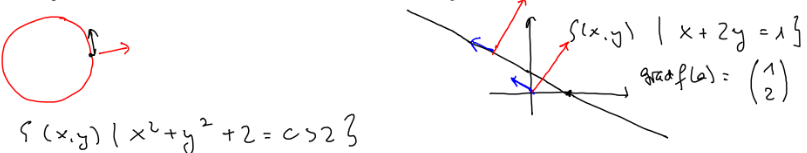
\includegraphics[width=0.8\linewidth]{erinnerung_niveauflaeche_intuition}
    \label{fig:erinnerung_niveauflaeche_intuition}
  \end{figure}
  Satz über implizite Funktion: 
  \begin{figure}[H]
    \centering
    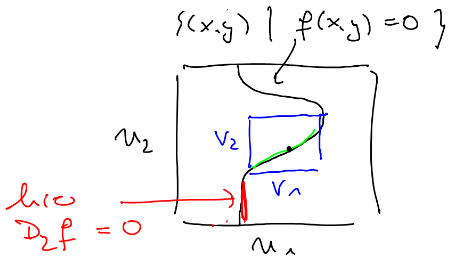
\includegraphics[width=0.5\linewidth]{satz_implizite_funktion_erinnerung_intuition}
    \caption*{\( f\maps U_1\times U_2 \to \reals \). Niveaumenge kann lokal als Graph geschrieben werden, wenn \( D_2 f(a,b) \) invertierbar ist. \textcolor{red}{Weitere Erklärungen \tto Audio}.}
    \label{fig:satz_implizite_funktion_erinnerung_intuition}
  \end{figure}
\end{erinnerung*}
\begin{aufwaermuebung*}
  Sei \( \gamma\maps I\to \reals^3 \) differenzierbare Kurve.
  \begin{figure}[H]
    \centering
    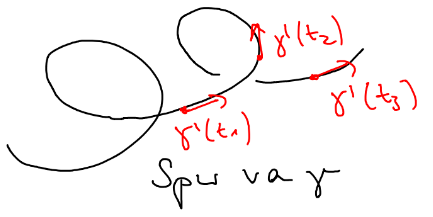
\includegraphics[width=0.5\linewidth]{spur_einer_kurve_auf_mannigfaltigkeit}
    \label{fig:spur_einer_kurve_auf_mannigfaltigkeit}
  \end{figure}
  Dann ist \( \gamma'(t) \) der \emph{Geschwindigkeitsvektor}, der sich im Punkt \( \gamma(t) \) auf die Kurve schmiegt.
\end{aufwaermuebung*}
\begin{beispiel*}
  \( f\maps I\to \reals \) differenzierbare Funktion. Betrachte \( \gamma(t)\definedas (t,f(t)) \). Also Spur von \( \gamma=\Gamma_f \). \( \gamma'(t)=(1,f'(t)) \).
  \begin{figure}[H]
    \centering
    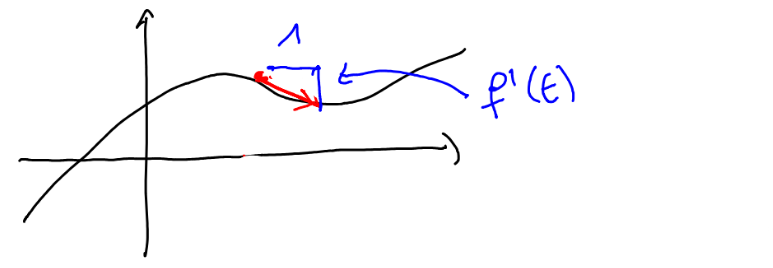
\includegraphics[width=0.5\linewidth]{graph_als_kurve_auf_mannigfaltigkeit}
    \label{fig:graph_als_kurve_auf_mannigfaltigkeit}
  \end{figure}
\end{beispiel*}
\begin{definition}\label{untermannigfaltigkeit}
  Eine Teilmenge \( M\subset \reals^n \) heißt \( d \)-dimensionale differenzierbare \emph{Unter-Mannigfaltigkeit} (oder reguläre Fläche) des \( \reals^n \), falls es für jedes \( a\in M \) eine Umgebung \( U\subset \reals^n \) von \( a \) gibt und eine stetig differenzierbare Abbildung \( f\maps U\to \reals^{n-d} \) \sd \begin{eigenschaftenenumerate}
    \item \label{untermannigfaltigkeit:ist_niveaumenge}\( M\cap U=\set{x\in U|f(x)=0} \) und 
    \item \label{untermannigfaltigkeit:maximaler_rang_gibt_dimension} \( \rang-{Df(a)}=n-d \) (maximal).
  \end{eigenschaftenenumerate}
  Das heißt \( M \) lässt sic lokal als Nullstellengebilde von \( n-d \) \( \reals \)-wertigen \( \stetigefunktionen[1] \) Funktionen \( f_j \) schreiben, deren Gradienten linear unabhängig sind.
  \begin{figure}[H]
    \centering
    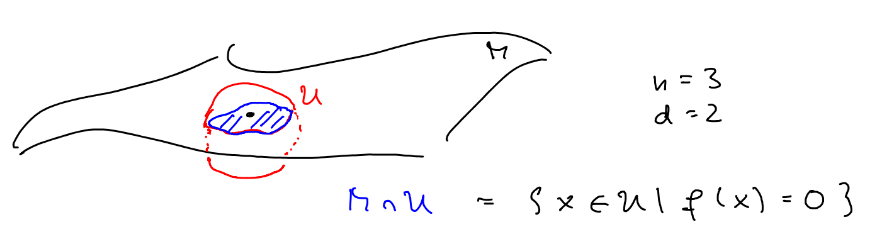
\includegraphics[width=0.5\linewidth]{untermannigfaltigkeit_intuition}
    \label{fig:untermannigfaltigkeit_intuition}
  \end{figure}
\end{definition}
\begin{beispiele*}
  \begin{enumerate}
    \item \label{untermannigfaltigkeit:beispiele:maximale_dimension:offene_teilmengen}Die \( n \)-dimensionalen Untermannigfaltigkeiten des \( \reals^n \) sind die offenen Teilmengen. Hier ist
    \begin{equation*}
      M\cap U=U=\Set{x\in U}.
    \end{equation*}
    \item\label{untermannigfaltigkeit:beispiele:ebene_4d} Ebene
    \begin{equation*}
      E=\set{p+(s,t,0,0)|s,t\in \reals}\subset \reals^4,
    \end{equation*}
    \( p\in \reals^4 \).
    \begin{figure}[H]
      \centering
      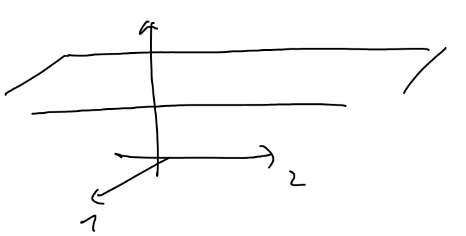
\includegraphics[width=0.5\linewidth]{langweilige_ebene_als_untermannigfaltigkeit}
      \caption*{Eine Dimension im Bild unterdrückt.}
      \label{fig:langweilige_ebene_als_untermannigfaltigkeit}
    \end{figure}
    Zu \( a\in E \) wähle \( U=\reals^4 \) und setze
    \begin{align*}
      f_1&\maps U\to \reals & f_1(x)&=\scalarproduct{x-p}{e_3}=x_3-p_3\\
      f_1&\maps U\to \reals & f_1(x)&=\scalarproduct{x-p}{e_4}=x_4-p_4.
    \end{align*}
    Es gilt \( x\in E \) \tiff \( f(x)=\begin{pNiceMatrix} f_1(x) \\ f_2(x) \end{pNiceMatrix}=0 \) und \( Df(a)=\begin{pNiceMatrix}
      0 & 0 & 1 & 0 \\ 0 & 0 & 0 & 1
    \end{pNiceMatrix} \), \( \rang-{}=2 \).
    \begin{figure}[H]
      \centering
      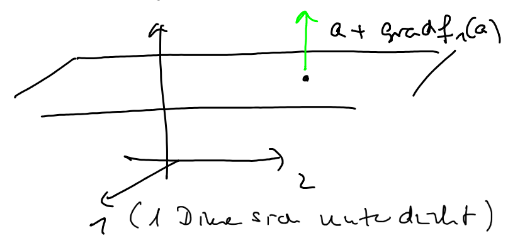
\includegraphics[width=0.5\linewidth]{normalenvektor_auf_langweiliger_ebene_als_untermannigfaltigkeit}
      \label{fig:normalenvektor_auf_langweiliger_ebene_als_untermannigfaltigkeit}
      \begin{equation*}
        \grad-{f_1}(a)=\begin{pNiceMatrix} 0 \\ 0 \\ 1 \\ 0 \end{pNiceMatrix}\qquad \grad-{f_2}(a)=\begin{pNiceMatrix} 0 \\ 0 \\ 0 \\ 1 \end{pNiceMatrix}.
      \end{equation*}
    \end{figure}
    Niveau-Mengen von \( f \):
    \begin{equation*}
      N_f(c)=\Set{x\in \reals^n|x_3-p_3=c,\logicspace x_4-p_4=c}.
    \end{equation*}
    \begin{figure}[H]
      \centering
      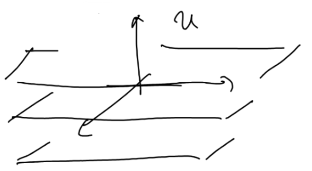
\includegraphics[width=0.5\linewidth]{normalenvektor_auf_langweiliger_ebene_als_niveaumengen}
      \caption*{\( N_f(0)=E \), Gradient steht senkrecht.}
      \label{fig:normalenvektor_auf_langweiliger_ebene_als_niveaumengen}
    \end{figure}
    \item \label{untermannigfaltigkeit:beispiele:sphaere}\( \mathbb{S}^{n-1}\definedas \Set{x\in \reals^n|\euclidiannorm{x}=1} \). Einheits-Sphäre. Zu \( a\in \mathbb{S}^{n-1} \) wähle \( U=\reals^n \) und \( f(x)=\euclidiannorm{x}^2-1 \). 
    \begin{equation*}
      Df(a)=(2a_1,\dotsc,2a_n)\neq 0.,
    \end{equation*}
    also \( \rang-{}=1 \forall a\in \mathbb{S}^{n-1}\).
    \item Eine \( 1 \)-dimensionale differenzierbare Untermannigfaltigkeit wird auch unparametisierte differenzierbare Kurve genannt. 
    \begin{beispiel*}
      \( f\maps \reals^3\to \reals^2 \).
      \begin{equation*}
        f(x,y,z)=\begin{pNiceMatrix} x^2+y^2+z^2-R^2 \\ x^2+y^2-r^2 \end{pNiceMatrix}\qquad R>r>0.
      \end{equation*}
      \begin{figure}[H]
        \centering
        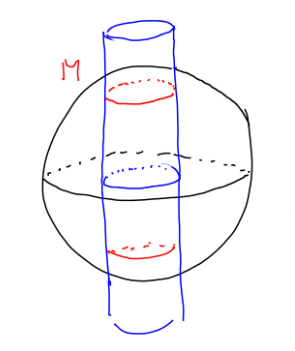
\includegraphics[width=0.5\linewidth]{zwei_kreise_auf_kugel_und_zylinder_als_untermannigfalteigkeit}
        \caption*{\textcolor{red}{\( M=\Set{(x,y,z)|f(x,y,z)=0}=N_f(0) \)}}
        \label{fig:zwei_kreise_auf_kugel_und_zylinder_als_untermannigfalteigkeit}
      \end{figure}
      \begin{equation*}
        Df(x,y,z)=\begin{pNiceMatrix} 2x & 2y & 2z \\ 2x & 2y & 0 \end{pNiceMatrix}
      \end{equation*}
      hat maximalen Rang \( 2 \) für \( z\neq 0 \) und \( (x,y)\neq 0 \).

      Letzteres ist für alle \( a\in M \) gewährleistet, weil \( (x^2+y^2=r^2>0) \) gilt und somit ist auch ersteres gewährleistet, da \( z^2=-r^2+R^2>0 \).

      Man sieht auch direkt: Die Funktion, die \( M \) lokal als Nullstellenmenge beschreibt, ist nicht eindeutig: \zb
      \begin{equation*}
        \tilde{f}(x,y,z)=\begin{pNiceMatrix} z^2+r^2-R^2 \\ x^2+y^2-r^2 \end{pNiceMatrix}
      \end{equation*}
      beschreibt im Beispiel oben das selbe \( M \).
    \end{beispiel*}
  \end{enumerate}
\end{beispiele*}
\begin{definition}\label{tangentialraum}
  Ein Vektor \( v\in \reals^n \) heißt \emph{Tangentialvektor} der Untermannigfaltigkeit \( M\subset \reals^n \) im Punkt \( a \), falls \texists differenzierbare Kurve \( \gamma \), \( \gamma\maps \ointerval{-\varepsilon}{\varepsilon} \to M\), \sd \( \gamma(0)=a \) und \( v=\gamma'(0) \). Die Menge der Tangentialvektoren im Punkt \( a \) bezeichnet man mit \( \tangentialraum-{M} \). 
  \begin{figure}[H]
    \centering
    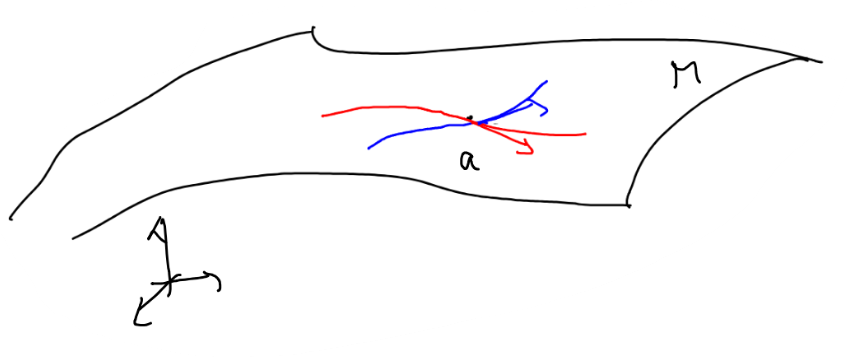
\includegraphics[width=0.5\linewidth]{tangentenvektoren_intuition}
    \caption*{Man zeichnet Tangentialvektoren an den Punkt \( a \) an. Aber eigentlich sind es \emph{keine} affinen Vektoren.}
    \label{fig:tangentenvektoren_intuition}
  \end{figure}
\end{definition}
\begin{beispiele*}
  \begin{enumerate}
    \item Ebene
    \begin{equation*}
      E=\set{p+(s,t,0,0)|s,t\in \reals}\subset \reals^4,
    \end{equation*}
    \( p\in \reals^4 \), \( a\in E \).
    \begin{equation*}
      \tangentialraum-{M}=\Set{v\in \reals^4|v=v_1e_2+v_2e_2},
    \end{equation*}
    denn jedes \( \gamma\maps \ointerval{-\varepsilon}{\varepsilon}\to M \) mit \( \gamma(0) \) ist von der FOrm
    \begin{equation*}
      \gamma(t)=a+(\tilde{\gamma}_1(t),\tilde{\gamma}_2(t),0,0).
    \end{equation*}
    Man zeichnet den Tangentialraum an der Stelle \( a \) ein, also
    \begin{figure}[H]
      \centering
      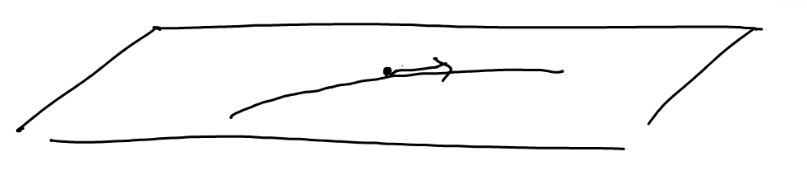
\includegraphics[width=0.5\linewidth]{tangentialvektor_an_ebene}
      \label{fig:tangentialvektor_an_ebene}
    \end{figure}
    \item \( M=\mathbf{S}^{n-1} \). Behauptung: 
    \begin{figure}[H]
      \centering
      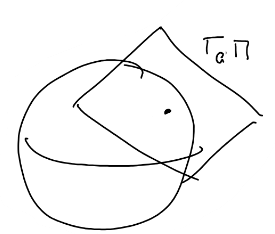
\includegraphics[width=0.5\linewidth]{tangentialraum_an_kugel}
      \label{fig:tangentialraum_an_kugel}
    \end{figure}
    Das erklärt den Namen: Die Tangentialvektoren sind tangential (angeschmiegt) an \( M \) im Punkt \( a \).
    
    Zum Beweis der Behauptung beweisen wir allgemeiner:
  \end{enumerate}
\end{beispiele*}
\begin{satz}\label{tangentialraum_ist_tangential}
  \approxtimestamp{24}
  Sei \( M \) \( d \)-dimensionale differenzierbare Untermannigfaltigkeit des \( \reals^n \). Ist 
  \begin{equation*}
    a\in M\cap U =\set{x\in U |f(x)=0}
  \end{equation*}
  für eine Funktion \( f\maps U\to \reals^{n-d} \) wie in \thref{untermannigfaltigkeit}, also \( Df(a) \) von maximalem Rang (\( n-d \)). Dann ist \( \tangentialraum-{M}=\ker-{Df(a)} \). Insbesondere ist \( \tangentialraum-{M} \) Untervektorraum von \( \reals^n \).
\end{satz}
\begin{proof}
  \begin{proofdescription}
    \item[\enquote{\( \subset \)}] Sei \( \gamma\maps \ointerval{-\varepsilon}{\varepsilon}\to M\cap U \) mit \( \gamma(0)=a \), \( \gamma'(0)=v \). Dann ist 
    \begin{equation*}
      0=\evaluateat{\frac{\differential}{\differential t} f\circ \gamma(t)}{t=0}=Df(\gamma(0))\matrixmult \gamma'(0)=Df(a)\matrixmult v\implies v\in \ker-{Df(a)}.
    \end{equation*}
    \item[\enquote{\( \supset \)}] Beweisen wir später mit Hilfe des folgenden Satzes~\ref{untermannigfaltigkeit_kriterium}.
  \end{proofdescription}  
\end{proof}
\begin{interpretation*}[für \( n-d=1 \)]
  Der Gradient zeigt in die Richtung des stärksten Anstiegs von \( f \). Eine Kurve \( \gamma \) wi in \ref{tangentialraum} (und \ref{tangentialraum_ist_tangential}) verläuft in einer Niveaumenge von \( f \) (und zwar hier zu \( c=0 \)). In Richtung \( v=\gamma'(0) \) ändert sich \( f \) also nicht und die Richtungsableitung in Richtung \( v \) ist \( 0 \):
  \begin{equation*}
    \partial_v f(a)=\scalarproduct{v}{\grad-{f}(a)}=Df(a)\matrixmult v=0\qquad (\text{\thref{tangentialraum_ist_tangential}}),
  \end{equation*}
  also \( v\perp \grad-{f}(a) \). \enquote{Der Gradient steht auf Niveaumengen senkrecht}.
\end{interpretation*}
\begin{beispiel*}
  \( f(x,y)=x^2+y^2-2 \). \( M= \) Niveaumenge \( N_f(0)=\set{x^2+y^2=2} \). \( \grad-{f}(a)=2(a_1,a_2) \).
  \begin{figure}[H]
    \centering
    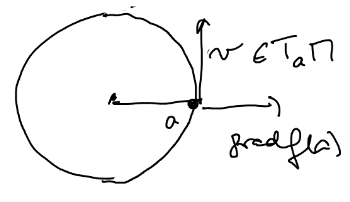
\includegraphics[width=0.5\linewidth]{tangentialraum_an_kreis_ist_tangential}
    \label{fig:tangentialraum_an_kreis_ist_tangential}
  \end{figure}
  Eine Kurve, die in \( M \) verläuft und für die gilt
  \begin{equation*}
    \gamma(0)=a=\begin{pNiceMatrix} \sqrt{2} \\ 0 \end{pNiceMatrix} 
  \end{equation*}
  ist
  \begin{equation*}
    \gamma(t)=\begin{pNiceMatrix} \Cos-{t} \\ \Sin-{t} \end{pNiceMatrix}\cdot \sqrt{2}.
  \end{equation*}
  Es ist dann
  \begin{equation*}
    \gamma'(0)=\sqrt{2}\begin{pNiceMatrix} 0 \\ 1 \end{pNiceMatrix}\perp \grad-{f}\begin{pNiceMatrix} \sqrt{2} \\ 0 \end{pNiceMatrix}=\begin{pNiceMatrix} 2\sqrt{2} \\ 0 \end{pNiceMatrix}.
  \end{equation*}
  \minisec{Höher-dimensionale Sphären:}
  \( N_f(0) \), \( f(x)=\euclidiannorm{x}^2-1 \). \( Df(a)=2(a_1,\dotsc,a_n) \). \( \ker-{Df}(a)= \) Ebene senkrecht zu \( a \).
  \begin{figure}[H]
    \centering
    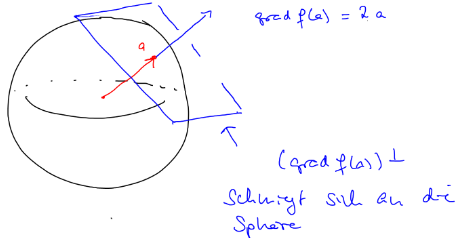
\includegraphics[width=0.5\linewidth]{tangentialraum_an_sphaere_ist_tangential}
    \label{fig:tangentialraum_an_sphaere_ist_tangential}
  \end{figure}
  Um di Rückrichtung von \thref{tangentialraum_ist_tangential} beweisen zu können, benötigen wir eine weitere (äquivalente) Charakterisierung differenzierbarer Untermannigfaltigkeiten.
\end{beispiel*}
\begin{satz}\label{untermannigfaltigkeit_kriterium}
  Eine Teilmenge \( M\subset \reals^n \) ist genau dann \( d \)-dimensionale differenzierbare Untermannigfaltigkeit des \( \reals^n \), wenn es zu jedem Punkt \( a\in M \) (nach eventueller Umnummerierung) Umgebungen \( V_1\subset \reals^d \) von \( a'=(a_1,\dotsc,a_d) \) un \( V_2\subset \reals^{n-d} \) von \( a''=(a_{d+1},\dotsc,a_n) \) und eine stetig differenzierbare Abbildung \( g\maps V_1\to \reals^{n-d} \), \( g(V_1)\subset V_2 \) gibt, \sd
  \begin{equation*}
    M\cap (V_1\times V_2)=\Gamma_g = \Set{(x',g(x'))|x'\in V_1}.
  \end{equation*}
\end{satz}
\begin{proof}
  \begin{proofdescription}
    \item[\hin] Sei \( a\in M \), \( U \), \( f \) wie in \thref{untermannigfaltigkeit}, insbesondere \( \rang-{Df(a)}=n-d \) (maximal) \timplies nach eventueller Umnummerierung ist \( Df(x',x'') \) für \( x=(x',x'')\in U\subset \reals^d \times\reals^{n-d} \)
    \begin{equation*}
      \begin{pNiceMatrix}[last-row]
        \partial_1 f_1(x' ,x'') & \Cdots & \partial_d f_1(x'.x'') & \partial_{d+1}f_1(x',x'')&\Cdots \partial_n f_1(x',x'') \\
        \Vdots &  & \Vdots & \Vdots & & \Vdots  \\
         \partial_1 f_{n-d}(x' ,x'') & \Cdots & \partial_d f_{n-d}(x'.x'') & \partial_{d+1}f_{n-d}(x',x'')&\Cdots \partial_n f_{n-d}(x',x'')\\
         &&&\Hdotsfor{3}_{D_2f(x'.x'')}
      \end{pNiceMatrix},
    \end{equation*}
    \sd \( D_2f(a',a'') \) invertierbar ist.

    Zudem ist \( f(a)=0 \). Der Satz über implizite Funktion liefert also eine lokale Auflösung von \( N_f(0) \) \timplies \Beh.

    \item[\rueck] Sei 
    \begin{equation*}
      M\cap V_1\times V_2=\Set{(x',g(x'))|x'\in V_1},
    \end{equation*}
    \( V_1\subset \reals^d \), \( V_2\subset \reals^{n-d} \). Setze
    \begin{gather*}
      f\maps V_1\times V_2\to \reals^{n-d}\\
      f_j(x',x'')=g_j(x')-x_j''.
    \end{gather*}
   Dann ist \end{proofdescription}  
   \begin{equation*}
     M\cap V_1\times V_2=\set{x\in V_1\times V_2|f(x)=0}
   \end{equation*}
   und
   \begin{equation*}
     Df(x)=\begin{pNiceArray}{CCC|CCC}[first-col]
       & \partial_1 g_1(x) & \Cdots & \partial_d g_1(x) & -1 & & 0 \\
       & \Vdots &  & \Vdots &  &\Ddots &  \\
       & \partial_1 g_{n-d}(x) & \Cdots & \partial_d g_{n-d}(x) & 0 & & -1 \\
     \end{pNiceArray}
   \end{equation*}
   hat maimalen Rang (\( n-d \)).
\end{proof}
\begin{bemerkung*}
  Man kann also eine \( d \)-dimensionale differenzierbare Untermannigfaltigkeit lokal stets als Graphen einer \( \stetigefunktionen[1] \)-FUnktion schreiben.

  Für die Beispiele oben gilt
  \begin{description}
    \item[\ref{untermannigfaltigkeit:beispiele:maximale_dimension:offene_teilmengen}] \( U\subset \reals^n \) offen, \( V_2=\emptyset \), \( V_1=U \).
    \item[\ref{untermannigfaltigkeit:beispiele:ebene_4d}] Ebene
    \begin{equation*}
      E=\set{p+s e_1+t e_2|s,t\in \reals}\subset \reals^4,
    \end{equation*}
    \( p\in \reals^4 \).
    \begin{equation*}
      g\maps \reals^2\to \reals^2\qquad g(x_1,x_2)=\begin{pNiceMatrix} p_3 \\ p_4 \end{pNiceMatrix}
    \end{equation*}
    konstant.
    \begin{figure}[H]
      \centering
      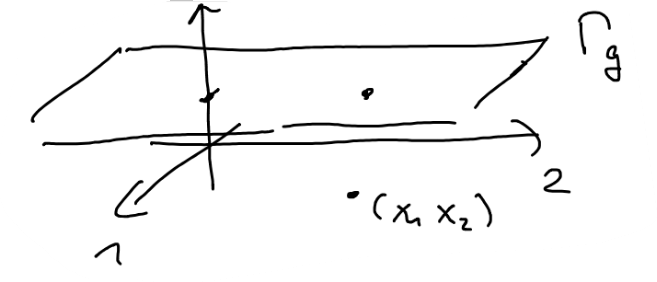
\includegraphics[width=0.5\linewidth]{langweilige_ebene_als_graph}
      \label{fig:langweilige_ebene_als_graph}
    \end{figure}
    \item[\ref{untermannigfaltigkeit:beispiele:sphaere}] \( \mathbf{S}^{n-1} \): Sei \( a\in \mathbf{S}^{n-1} \) mit \( a_n>0 \). Sei
    \begin{gather*}
      V_1=\Set{x'\in \reals^{n-1}|\euclidiannorm{x'}<1}\\
      g\maps V_1\to \reals,\qquad g(x_1,\dotsc,x_{n-1})=\sqrt{1-x_1^2--\dotsb-x_{n-1}^2}.
    \end{gather*}
    Dann ist
    \begin{equation*}
      \mathbf{S}^{n-1}\cap V_1\times \ointerval{0}{\infty}=\Gamma_g.
    \end{equation*}
    \begin{figure}[H]
      \centering
      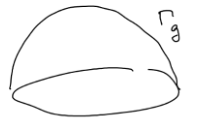
\includegraphics[width=0.5\linewidth]{halbsphaere_als_graph}
      \label{fig:halbsphaere_als_graph}
    \end{figure}
  \end{description}
\end{bemerkung*}\approxtimestamp{40}
\begin{proof}[Fortsetzung Beweis \thref{tangentialraum_ist_tangential}]
  Wir beweisen nun die zweite Inklusion von \thref{tangentialraum_ist_tangential}, also \( \tangentialraum-{M}\supset \ker-{Df(a)} \). Sei \( g\maps V_1\to \reals^{n-d} \) stetig differenzierbar \sd \( g(V_1)\subset V_2 \) und \( a\in V_1\times V_2\subset \reals^d \times \reals^{n-d} \) und
\begin{equation*}
  M\cap (V_1\times V_2)=\Gamma_g=\Set{(x,g(x))|x\in V_1}.
\end{equation*}
Sei \( x_0\in V_1  \) \sd \( (x_0,g(x_0))=a \). Betrachte \( \varphi\maps V_1\to \reals^n \), \( \varphi(x)=(x,g(x)) \). Dann ist
\begin{equation*}
  D\varphi(x_0)\matrixmult v\explain{\text{Kettenregel}}{=}\evaluateat{\frac{\differential}{\differential t} \varphi(x_0+tv)}{t=0}\qquad \forall v\in \reals^d.
\end{equation*}
\timplies \( a=\varphi(x-0) \) und 
\begin{equation*}
  w\definedas \evaluateat{\frac{\differential}{\differential t} \varphi(x_0+tv)}{t=0}\in \tangentialraum-{M},
\end{equation*}
also \( \image{D\varphi(x_0)}\subset \tangentialraum-{M} \). Zudem wissen wir schon: \( \tangentialraum-{M}\subset \ker-{Df(a)} \). Es ist \( D\varphi(x_0)\maps \reals^d\to \reals^n \), \( D\varphi(x_0)=\begin{pNiceMatrix} \mathds{1}_{d\times d} \\ Dg(x_0) \end{pNiceMatrix} \), also injektiv \timplies (Dimensionsformel)
\begin{equation*}
  \dim-{}{\image{D\varphi(x_0)}}=d=n-\underbrace{\rang-{Df(a)}}_{=n-d}=\dim-{}{\ker-{Df(a)}}
\end{equation*}
\timplies \( \tangentialraum-{M}=\ker-{Df(a)} \).
\end{proof}
Wir haben im Beweis auch gesehen:
\begin{equation*}
  \tangentialraum-{M}=\image-{D\varphi(x_0)},
\end{equation*}
wo \( \phi(x)=\transpose-{(x,g(x))} \) die Graphenabbildung einer lokalen Auflösung \( g \) ist it \( a=\transpose-{(x_0,g(x_0))}=\phi(x_0) \).

Die geometrische Interpretation ist:
\begin{figure}[H]
  \centering
  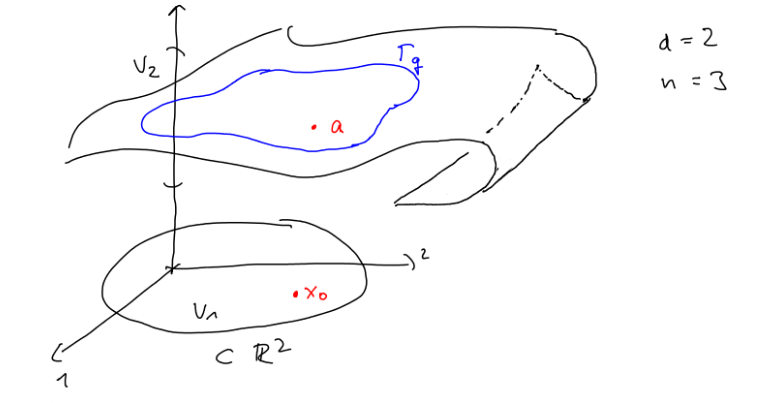
\includegraphics[width=0.5\linewidth]{setup_interpretation_bild_ableitung_implizite_funktion}
  \label{fig:setup_interpretation_bild_ableitung_implizite_funktion}
\end{figure}
\begin{equation*}
  D\phi(x_0)=\explain{\partial_1 g(x_0)\logicspace  \partial_2 g(x_0)}{\begin{pNiceMatrix} \mathds{1}_2 \\ Dg(x_0) \end{pNiceMatrix}}.
\end{equation*}
Die Spalten von \( D\phi(x_0) \) 
\begin{equation*}
  \explain[Big]{\text{Veränderug von \( g \) in \( 1 \)-Richtung}}{\begin{pNiceMatrix} 1 \\ 0 \\ \partial_1 g(x_0) \end{pNiceMatrix}}\logicspace \text{und}\logicspace \explain{\text{Veränderung in \( 2 \)-Richtung}}{\begin{pNiceMatrix} 0 \\ 1 \\ \partial_2 g(x_0) \end{pNiceMatrix}}
\end{equation*}
\begin{figure}[H]
  \centering
  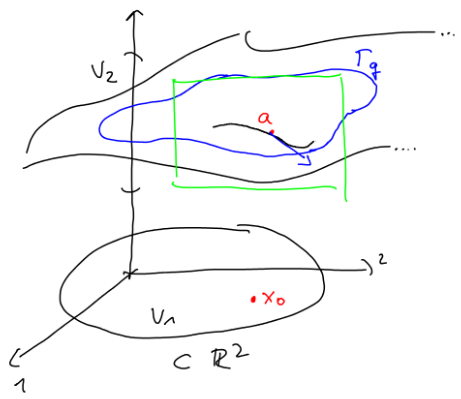
\includegraphics[width=0.5\linewidth]{interpretation_bild_ableitung_implizite_funktion}
  \caption*{\textcolor{green}{Ebene parallel zur \( 2 \)-\( 3 \)-Ebene durch \( a \)\( =\set{x_1=x_{0,1} \text{ konstant}} \)}. 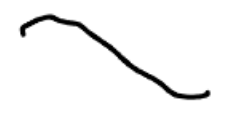
\includegraphics[height=\baselineskip]{little_line}\( =\Set{(x_{0,1},x_{0,2}+t,g(x_{0,1},x_{0,2}+t))|t\in I\subset \reals} \) ist Kurve in \( M \).}
  \label{fig:interpretation_bild_ableitung_implizite_funktion}
\end{figure}
Ableitung
\begin{equation*}
  \frac{\differential}{\differential t}\phi(x_{0,1},x_{0,2}+t)=(0,1,\partial_2 g(x_{0,1},x_{0,2}+t)).
\end{equation*}
Es gilt \( \evaluateat{\phi(x_{0,1},x_{0,2}+t)}{t} \) und \( (0,1,\partial_2g(x_0)) \) ist \textcolor{blue}{Tangentialvektor} bei \( a \). Genauso für die Ebene \( \set{x_2=x_{0,2}} \) und die erste Spalte von \( D\phi(x_0) \). Jede \( d\)-dimensionale Untermannigfaltigkeit lässt sich lokal zu einer Teilmenge einer \( d \)-dimensionalen Ebene im \( \reals^n \) \enquote{plätten},
\begin{satz}\label{mannigfaltigkeit_sieht_lokal_aus_wie_r_n}
  \( M\subset \reals^n \) ist genau dann \( d \)-dimensionale Untermannigfaltigkeit, wenn es zu jedem Punkt \( a\in M \) offene Umgebungen \( U \) von \( a\subset \reals^n \) und \( V \) von \( 0\subset \reals^n \) und einen \emph{Diffeomorphismus} von \( U \) nach \( V \), also eine stetig differenzierbare invertierbare Funktion \( F\maps U\to \reals^n \) mit stetig differenzierbarer Umkehrfunktion \( G\maps V\to \reals^n \) \sd 
  \begin{equation*}
    F(M\cap U)=\Set{(y',y'')\in \reals^d\times \reals^{n-d}|y''=0}\cap V.
  \end{equation*}
  \begin{figure}[H]
    \centering
    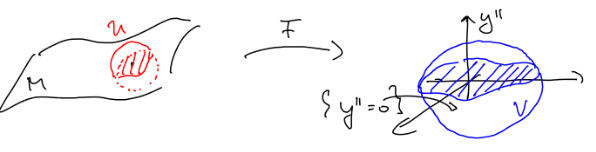
\includegraphics[width=0.5\linewidth]{mannigfaltigkeit_sieht_lokal_aus_wie_r_n}
    \label{fig:mannigfaltigkeit_sieht_lokal_aus_wie_r_n}
  \end{figure}
\end{satz}
\begin{proof}
  \begin{proofdescription}
    \item[\hin] Sei \( M \) in einer Umgebung von \( a \) als Graph dargestellt (\texists nach \thref{untermannigfaltigkeit_kriterium}),
    \begin{equation*}
      M\cap (V_1\times V_2)=\set{(x',g(x'))|x'\in V_1}
    \end{equation*}
    Setze \( U\definedas V_1\times V_2 \) und \( F(x,x'')=(x',x''-g(x')) \). \( F \) ist stetig differenzierbar und die Umkehrfunktion
    \begin{equation*}
      \inverse{F}(y',y'')=(y',y''+g(y'))
    \end{equation*}
    ist ebenfalls stetig differenzierbar, \( \inverse{F}\maps F(U)\to \reals^n \). \( F(U) \) ist offen nach \thref{offene_abbildungen_satz} weil
    \begin{equation*}
      DF(x'.x'')=\begin{pNiceMatrix}
        \mathds{1}_{d\times d} & -Dg(x') \\
        0 & \mathds{1}_{(n-d)\times (n-d)}
      \end{pNiceMatrix}
    \end{equation*}
    invertierbar ist für alle \( (x',x'')\in U \). Es ist \( F(M\cap U)=\Set{(x',0)|x'\in V_1} \).

    Es ist 
    \begin{equation*}
      F(M\cap U) =\set{(x',0)|x'\in V_1}.
    \end{equation*}
    \item[\rueck] Sei \( F\maps U\to \reals^n \) Diffeomorphismus, \( F(U)=V \), mit 
    \begin{equation*}
      F(M\cap U)=\Set{y\in V|y_{d+1}=\dotsb=y_n=0}.
    \end{equation*}
    Dann ist
    \begin{align*}
      M\cap U&=\inv{F}\parens*{\Set{y\in V|y_{d+1}=\dotsb=y_n=0}}\\
      &=\set{x\in U|F_{d+1}(x)=\dotsb=F_n(x)=0}.
    \end{align*}
    Der Ran von
    \begin{equation*}
      \begin{pNiceMatrix}
        \partial_1 F_{d+1}(a) & \Cdots & \partial_n I_{d+1}(a) \\
        \Vdots &  & \Vdots \\
        \partial_1 F_N(a) & \Cdots & \partial_n F_{d+1}(a)
      \end{pNiceMatrix}
    \end{equation*}
    ist maximal (also gleich \( n-d \)), weil die Ableitungsmatrix \( DF(a)\in \sqmatrices{n}{\reals} \) invertierbar ist \timplies \( M \) ist \( d \)-dimensionale Untermannigfaltigkeit.
  \end{proofdescription}
  
\end{proof}
\begin{beispiel*}
  \( \mathbb{S}^{n-1} \), \( a\in \mathbb{S}^{n-1} \), \( a_n>0 \). \( g\maps D\to \reals  \) mit \( D=\set{x\in \reals^{n-1}|\euclidiannorm{x}<1} \),
  \begin{equation*}
    g(x_1,\dotsc,x_{n-1})=\sqrt{1-\sum_{i=1}^{n-1}x_i^2}.
  \end{equation*}
  \( F\maps D\times \ointerval{0}{\infty}\to \reals^n \),
  \begin{equation*}
    F(x,t)=\parens*{x,t-\sqrt{1-\sum_{i=1}^{m_1}x_i^2}}.
  \end{equation*}
  \( \mathbb{S}^{n-1}\cap D\times \ointerval{0}{\infty}=
\includegraphics[height=\baselineskip]{kleine_offene_halbsphaere} \) (ohne den Rand 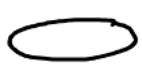
\includegraphics[height=\baselineskip]{kleiner_fehlender_rand}) und % ChkTeX 25
  \begin{equation*}
    F(M\cap D\times \ointerval{0}{\infty})=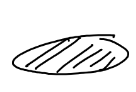
\includegraphics[height=\baselineskip]{kleine_geplaettete_offene_halbkugel}=D. % ChkTeX 25
  \end{equation*}
\end{beispiel*}